\graphicspath{{chapters/4.Chapter_2/figures}}

\begin{savequote}[75mm]
"even after the observation of the frequent or constant conjunction of objects, we have no reason to draw any inference concerning any object beyond those of which we have had experience;"
\qauthor{- David Hume: \textit{A Treastie of Human Nature, 1738}}
\end{savequote}


\chapter{Transcriptomic analysis of the \textit{Paramecium bursaria} and \textit{Micractinium reisseri} endosymbiosis}

Transcriptomics, and specifically RNA-Seq, are a powerful method by which the \textit{Paramecium bursaria}-\textit{Micractinium reisseri}
endosymbiosis can be investigated. Due to the photosynthetic basis of this endosymbiosis, a (relatively) unbiased
global metatranscriptomic profile of host and endosymbiont simultaneously in both lit and dark conditions can be used
to identify key transcripts involved its maintenance. This is evidenced by several studies (e.g. \citep{Nowack2011,Jiggins2013,Xiang2015}) using a similar approach
to investigate host-chloroplast interactions. These transcriptomic methods which fall between analysis of homogeneous single organism cultures and
large scale metatranscriptomics have been dubbed by some ``dual-RNAseq'' \citep{Westermann2012} and are exemplified by Tierney \textit{et. al.} in the context 
of eukaryote-eukaryote host-pathogen interactions \citep{Tieryney2012}.

\textit{Paramecium bursaria} - \textit{Micractinium reisseri} is well placed for a ``dual-RNAseq'' analysis as it has 




(even custom bioinformatics pipelines aimed at this host-pathogen ``dual-RNAseq'' analysis have been published \citep{Xu2015}).




However, there are several key difficulties in simultaneously profiling multiple organisms: first and foremost the identification
of transcript origins 




There are several key difficulties in applying this ``dual-RNAseq'' approach to the PbMr system: a relative paucity of
reference genomes and/or transcriptomes to aid assembly, 

Lack of other examples, the Kodama PbCv transcriptome filtered out endosymbiont reads.  


Identifying the provenance of assembled transcripts after assembly, this is particularly non-trivial due to potential
origins ranging from partially digested bacterial food species as well as standard run of the mill contamination
from reagents and sequencing operations.





However, as both target species - host and endosymbiont are eukaryotes the complication of mRNA enrichment 
is simplified due to the sufficiency of poly-A selection for this task (instead of rRNA depletion methods)

Determining the necessary sequencing depth is also difficult.



Unfortunately, due to the unforseen problem of generating sufficient culture density with the CCAP1660/12
strain bulk transcriptome methods were only able to generate a single day and night library.


To solve this, and specifically, to allow accurate inference of differential expression 




Therefore, the solution to this generated a new set of complications.


Interestingly, Westermann \textit{et. al.} observed that single-cell methodologies were a likely source of future
innovation in ``dual RNA-Seq'' studies \citep{Westermann2012}


First achieved in \citep{Lao2009}



\begin{itemize}
    \item 
    \item
    \item
    \item
\end{itemize}






It should also be noted that by only looking at transcripts that are differentially or generally highly expressed in both
day and night conditions we preclude the ability to discover necessary but constitutively expressed transcripts and necessarily
constitutively inhibited transcripts.  
Fortunately, to this end, the only other published 2nd generation sequencing analysis of \textit{P. bursaria} and a green algal,
endosymbiont: Kodama \textit{et. al.} 2014 \citep{Kodama2014} partially addressed this issue.  This analysis investigated 
the differential global metatranscriptome profile of \textit{P. bursaria} Yad1g strain with and without its \textit{Chlorella variabilis} 1N endosymbiont 
\citep{Kodama2014}.   While, this is a different strain of both host and endosymbiont to the CCAP1660/12 strains (\textit{P. bursaria} and \textit{Micractinium reisseri}) 
used in this thesis it offers a potential avenue to investigate these other components.
An attempt was made to replicate this work using the CCAP1660/12 strains, unfortunately, elimination of the endosymbionts without death of the host
didn't prove possible in these strains.  Despite using 

(despite earlier publications to the contrary) by either maintaining the culture in the dark \citep{Siegel1960} (although some studies have thrown doubt on
    how effective this method is at completely elimiating the photobiont \citep{Tanaka2002}) or treatment with various titrations of herbicides 
    (e.g. paraquat \citep{Hosoya1995a}) or the protein synthesis inhibitor cyclohexamide \citep{weis1984effect}).\footnote{
There are naturally aposymbiotic strains of \textit{Paramecium bursaria} \citep{Tonooka2002a}}













Towards this end we conducted a bulk RNA-Seq sequencing of cultured PbMr, unfortunately due to limitations in the quantity of
extracted RNA and maintainable culture density it was necessary to pool biological replicate day and night samples into single
day and night samples.  Therefore, to facilitate accurate inference of differential expression 
a number of day and night replicates were also sequenced using single-cell RNA-Seq (scRNA-Seq) methods.
To aid with transcriptome assembly and investigate the presence of genes that are not expressed in host
or endosymbiont during endosymbiosis.  This can be used combined with transcriptome data from 



Therefore, this chapter addresses the key difficulties of recapitulating the metatranscriptome and metagenome of \textit{Paramecium bursaria}
and \textit{Micractinium reisseri} from 2nd generation sequencing datasets (high-throughput short-reads), filtering unavoidable contamination
in the form of bacterial food species (and potentially endosymbionts) and viruses, utilising single cell approaches,
and identifying the provenance of assembled sequences, specifically whether they derive from host or endosymbiont.



%%Can you separate transcripts from host, endosymbiont and food bacteria?
%Current practices and how they were applied - BLAST, GC etc
%Initial binning vs phylogenetics - seems better
%But still too work intensive - use manually done 10,000 for rest of transcriptome therefore ML
%Flowchart of tool 
%t-SNE plot of vectors
%classifier log-loss and learning curve comparison using logistic regression, SVM with diff kernels
%Convergence check for SVM hyperparameters
%anomaly detection?
%
%Transcriptome Assembly:
%
%- Trimming: MacManes 5, 30 (also did 12 and 35)
%- Error correction: Spades error correction
%- GC clustering parKour

%%Abstract intro - in order to interrogate a system need to assemble the transcripts corresponding
%to them 

\section{Sample Preparation and Sequencing}

\subsection{Bulk transcriptomic RNA preparation}
For bulk transcriptomic analyses CCAP 1660/12 cells were harvested in a way to minimise the 
number of bacterial prey species from the culture, \textasciitilde \(10^{6}\) 
cell aliquots were strained through \(40\mu m\) sieves, filtered on 
\(10 \mu m\) nylon filters, 
before finally being filtered on \(8 \mu m\) TETP polycarbonate filters using a 
low-pressure filtration pump.  Collected samples were either immediately 
quick-frozen in liquid nitrogen for storage (\(-20\)\celsius for short-term storage 
and \(-80\)\celsius for longer storage) or harvested by centrifugation.  
In order to investigate the two main metabolic states of the symbiosis 
(i.e. under light conditions during active photosynthesis and in the dark 
when no photosynthesis is taking place) samples were extracted 5 hours into 
the light and dark phase of the 12:12 hour day-night cycle.

To ensure extracted RNA was representative of healthy and interacting host 
and endosymbionts care was taken to minimise the number of dead/dying cells 
from which RNA was extracted.  In order to do this, a subsample was taken 
from each culture during the process of harvesting and scored for dead/dying cells.  
Cell assays were formed by taking 1-2ml of each harvest cell pellet and 
fixed using 40\(\mu l\) Lugol's solution (0.5g \(I_{2}\) and 1g KCl in 8.5ml 
of MilliQ water). Dead/dying cells were identified as broken or puckered cells 
and counted using light microscopy.  Samples containing >10\% dead/dying cells 
were discarded and no RNA extracted from them.

In order to lyse collected samples, cells were washed from the filter or the 
pellet was resuspended in 1ml TriReagent (Sigma) heated to \(60\)\celsius. 
Cells were vortexed with sterile \(300\mu m\) glass-beads for 15s, incubated at 
room temperature for 10 minute, vortexed for 15s, quick-frozen in liquid 
nitrogen and stored at \(-20^{o}C\) before further processing.  
Samples were defrosted, vortexed for 15s, placed in a heat-block set 
to \(60^{o}C\) for 10 minutes while continuing to be vortexed, removed from 
heating and vortexed again for 15s.  
RNA was extracted by adding 0.2ml of Chloroform to the glass-bead-trizol-sample 
solution, shaking for 15s, incubating for 5 minutes at room temperature and 
centrifuging at 12,000g for 15 minutes at $4^{o}$C.  
The upper-phase was then transferred to an RNAse-free 1.5ml tube and an 
equal volume (\textasciitilde$0.5$ml) of isopropanol was added before shaking for 15s.  
The isolated RNA was then incubated at $-20^{o}$C for 10 minutes 
(up to several hours) before being collected as a pellet using a centrifuge at 
10,000g for 10 minutes at $4^{o}$C (supernatant was discarded). 
The RNA pellet was then washed with 1ml of 75\% ethanol and centrifuged 
twice at 10,000g for 10 minutes at $4^{o}$C with the supernatant being 
discarded after each centrifugation.  
Pellet was dried before being resuspended in 100$\mu l$ of RNAse-free water.  
The RNA was then cleaned further using the Qiagen RNeasy clean-up kit 
before being assessed for quality using ND-1000 (NanoDrop) and BioAnalyzer (Agilent).

The bulk day and night library were paired-end \(76bp\) sequenced using an Illumina Genome
Analyzer II by the Exeter University Sequencing Service.  The two libraries were sequenced
on separate flowcells.

\subsection{Bulk Transcriptome Trimming}

FastX-toolkit adapative trimming Q20 applied by sequencing service.
Raw untrimmed FASTQ data not available




\subsection{Single Cell preparations}

For single cell transcriptomics, a ``cell-picking'' approach was used in which
\textit{P. bursaria} cells were inspected on an inverted light microscope before being picked
using an orally aspirated drawn-glass Pasteur pipette \citep{Garcia-Cuetos2012}.
In order to mininmise contamination from food bacteria present in the media these picked cells
were washed 3 times by serial transfer to \(10\mu l\) droplets of sterile NCL media.
The washed cell was then transferred to a \(10\mu l\) droplet of sterile water.

\subsubsection{Single Cell transcriptomic cDNA preparation}
Cells were transferred from their respective \(10\mu l\) droplets of sterile water to
a PCR tube containing \(6\mu l\) water and \(4\mu l \) lysis buffer (from the Qiagen
REPLI-g WTA Single Cell Kit). To disrupt the cell beads (Sigma, \(425-600\mu m\), acid-washed)
were added to the meniscus, before submersion in liquid nitrogen for 5 seconds.  The sample was 
then thawed before vortexing for 1 minute.  
mRNA was selectively amplified and reverse transcribed to cDNA using poly-A selection.  The cDNA
was then amplified using multiple displacement amplification and the amplified cDNA purified
using a QIAamp DNA mini kit eluted in \(100\mu l\) elution buffer.

%\subsubsection{Single Cell genomic DNA preparation}
%Cells were transferred from their respective \(10\mu l\) droplets of sterile water to a microncentrifuge tube.
%CTAB method adapted from \citep{Winnepenninckx1993}.  Cells were disrupted by vortexing for 5 minutes with
%\(748.5\mu l\) CTAB extraction buffer (at 37\celsius) and ceramic beads (Sigma, \(425-600\mu m\), acid-washed).
%The tube was then incubated for 50 minutes at 37\celsius, vortexed for 5 minutes, and incubated for a further 50
%minutes at 60\celsius. DNA was extracted 3 times using phenol, chloroform and isoamylalcohol at a 25:24:1 ratio (pH 8),
%washed with 70\% ethanol and re-suspended in \(2.5\mu l\) TE buffer (pH 8). This DNA then underwent 
%Multiple displacement-based whole genome amplification using the Repli-G Single Cell Kit before purification using a 
%QIAmp DNA mini kit before elution in \(100\mu l\) elution buffer.  

\subsubsection{Library preparation}

Each cDNA sample was fragmented in \(130\mu l\) 1xTE buffer on the Covaris E220 
with a target size of \(225bp\) (duty factor of \(10\%\), 200 cycles per burst, peak incident power
of 175, \(200s\) at \(7^{o}C\)). Fragment sizes were checked on a BioAnalyzer (Agilent) 7500 DNA chip.
cDNA was then concentrated using a GeneRead kit column with a elution in \(35\mu l\). Fragmentation
step was then repeated 3 times (\(110s\)) until majority of cDNA in each library was between \(200-250bp\)

cDNA ends were then end-repaired, adenylated and adapters ligated using the NEXTFlex (Biooscientfic) sequencing kit 
according to the manufacturer's instructions and using NEBNext (New England Biolabs) indices.  Also following
the NEXTFlex kit instructions, MgNa bead purification was done before and after PCR amplification using
NEBNext reagents.  Finally, prepared libraries were size selected using a Blue Pippin machine at a size selection
of \(350bp\) (range \(315-385bp\)).

A final bioanalyzer step was conducted with individual library concentrations ranging from \(0.66-4.09nM\).
All libraries 


\section{Transcriptome Assembly}

As mapping to even divergent (up to 15\%) genomes can generate transcriptomes of higher-quality
than de novo \citep{Vijay2013}

SCT


\subsection{Library Assessment}

For all sequencing project is is important to perform quality control on the sequenced libraries.
This is especially important for single 


As assemblies were observed to considerably worsen or improve depending on the exact 
SCT library inclusion.  I sought to get a rough approximation for possible differences between
the libraries and to investigate possible contamination.  For this purpose, I created a tool
christened "DueyDrop".

To achieve this 5 batches of 10,000 PE reads were sampled from each library after trimming %which trim?
using seqtk's \citep{SeqtkGitHub} reservoir sampling algorithm with a common seed used to sample paired
reads for the forward and reverse read files for each PE library in the same manner as trimming optimisation.

While 5 batches of 10,000 should be equivalent to 50,000 random samples by splitting sampling and using
a different random seed each time the risk of poor implementation of this randomisation algorithm is 
somewhat offset and standard deviations can be easily calculated to assess consistency of later results.

These random samples were subsequently used to query the NCBI Protein NR database via BLASTX as implemented
in Diamond.  A tool optimised for efficient BLASTing of short reads against larger databases.

The top hit for each read was kept and the GIs extracted.  Subsequently, these GIs were used to query
a local taxdump of the NCBI taxonomy database via BioPerl.

These taxonomic data were then tallied at multiple taxonomic levels summarised below.




\begin{table}[h]
\begin{tabular}{@{}|l|l|llllll@{}}
\toprule
\textbf{SCT Library} & \textit{\textbf{PE}} & \multicolumn{1}{l|}{\textbf{Eukaryote}} & \multicolumn{1}{l|}{\textbf{Bacteria}} & \multicolumn{1}{l|}{\textbf{Alveolate}} & \multicolumn{1}{l|}{\textbf{Viridiplantae}} & \multicolumn{1}{l|}{} & \multicolumn{1}{l|}{\textbf{Total Hits}} \\ \cmidrule(r){1-6} \cmidrule(l){8-8} 
\textit{Light1-9}    & \textit{R1}          & \multicolumn{1}{l|}{51.89 +/- 0.45}     & \multicolumn{1}{l|}{9.37 +/- 0.26}     & \multicolumn{1}{l|}{25.15 +/-  0.71}    & \multicolumn{1}{l|}{7.45 +/- 0.33}          & \multicolumn{1}{l|}{} & 69.49 +/- 0.37                           \\ \cmidrule(lr){2-2}
                     & \textit{R2}          & 51.75 +/- 0.25                          & 8.82 +/- 0.24                          & 24.85 +/- 0.56                          & 7.49 +/- 0.21                               &                       & 68.75 +/- 0.29                           \\ \cmidrule(r){1-2}
\textit{Light1-10}   & \textit{R1}          &                                         &                                        &                                         & \multicolumn{1}{l|}{}                       & \multicolumn{1}{l|}{} &                                          \\ \cmidrule(lr){2-2}
                     & \textit{R2}          &                                         &                                        &                                         &                                             &                       &                                          \\ \cmidrule(r){1-2}
\textit{Light1-11}   & \textit{R1}          &                                         &                                        &                                         & \multicolumn{1}{l|}{}                       & \multicolumn{1}{l|}{} &                                          \\ \cmidrule(lr){2-2}
                     & \textit{R2}          &                                         &                                        &                                         &                                             &                       &                                          \\ \cmidrule(r){1-2}
\textit{Dark1-2}     & \textit{R1}          &                                         &                                        &                                         & \multicolumn{1}{l|}{}                       & \multicolumn{1}{l|}{} &                                          \\ \cmidrule(lr){2-2}
                     & \textit{R2}          &                                         &                                        &                                         &                                             &                       &                                          \\ \cmidrule(r){1-2}
\textit{Dark1-3}     & \textit{R1}          &                                         &                                        &                                         & \multicolumn{1}{l|}{}                       & \multicolumn{1}{l|}{} &                                          \\ \cmidrule(lr){2-2}
                     & \textit{R2}          &                                         &                                        &                                         &                                             &                       &                                          \\ \cmidrule(r){1-2}
\textit{Dark1-5}     & \textit{R1}          &                                         &                                        &                                         & \multicolumn{1}{l|}{}                       & \multicolumn{1}{l|}{} &                                          \\ \cmidrule(lr){2-2}
                     & \textit{R2}          &                                         &                                        &                                         &                                             &                       &                                          \\ \cmidrule(r){1-2}
\textit{Dark2-2}     & \textit{R1}          &                                         &                                        &                                         & \multicolumn{1}{l|}{}                       & \multicolumn{1}{l|}{} &                                          \\ \cmidrule(lr){2-2}
                     & \textit{R2}          &                                         &                                        &                                         &                                             &                       &                                          \\ \cmidrule(r){1-2}
\textit{Dark2-3}     & \textit{R1}          &                                         &                                        &                                         & \multicolumn{1}{l|}{}                       & \multicolumn{1}{l|}{} &                                          \\ \cmidrule(lr){2-2}
                     & \textit{R2}          &                                         &                                        &                                         &                                             &                       &                                          \\ \cmidrule(r){1-2}
\textit{Dark2-6}     & \textit{R1}          &                                         &                                        &                                         & \multicolumn{1}{l|}{}                       & \multicolumn{1}{l|}{} &                                          \\ \cmidrule(lr){2-2}
                     & \textit{R2}          &                                         &                                        &                                         &                                             &                       &                                          \\ \cmidrule(r){1-2}
\textit{Dark2-7}     & \textit{R1}          &                                         &                                        &                                         & \multicolumn{1}{l|}{}                       & \multicolumn{1}{l|}{} &                                          \\ \cmidrule(lr){2-2}
                     & \textit{R2}          &                                         &                                        &                                         &                                             &                       &                                          \\ \cmidrule(r){1-2}
\textit{Dark2-8}     & \textit{R1}          &                                         &                                        &                                         & \multicolumn{1}{l|}{}                       & \multicolumn{1}{l|}{} &                                          \\ \cmidrule(lr){2-2} \cmidrule(l){7-8} 
                     & \textit{R2}          &                                         &                                        &                                         &                                             &                       &                                          \\ \cmidrule(r){1-2}
\end{tabular}
\end{table}



Scripts used to conduct this are available in my thesis scripts github repository:
\url{https://github.com/fmaguire/dueydrop}




\subsection{Trimming optimisation}

While there has been some analysis of optimal trimming for bulk RNA-Seq (particularly \citep{MacManes2014})
there has not been an investigation of the optimal trimming parameters for single cell RNA-Seq Illumina reads.
Correct trimming is important to minimise sequence error (mostly substitutions \citep{Yang2013}) as these
result in assembly of spurious sequences \citep{Macmanes2013,MacManes2014}


To determine optimal trimming parameters (\(\theta\)) for the raw single-cell paired-end RNA-Seq reads 
I used a naive grid search algorithm using random reads sub-sampled from each library and compared mapping
to bulk transcriptome assembly described above.
Specifically, 5000 PE reads were randomly sampled without replacement from each of the raw FASTQ libraries 
using the streaming reservoir sampling \citep{Vitter1985} algorithm implemented in Heng Li's 
seqtk C library (\citep{SeqtkGitHub}).
To guarantee the pairing was maintained the same random seed was used for the left and right read
of each library. This seed was subsequently incremented with each library sampled.
These random samples were subsequently trimmed using a variety of parameter values and combinations therein 
(see \ref{table:parameters} for details).
The trimmed samples were then mapped to the bulk RNA-Seq transcriptome reference dataset using bowtie2
\citep{Langmead2012} with maximum and minimum insert sizes of 37bp and 1161bp (derived from library preparation
fragment size distribution and histrogram of mapped insert sizes for untrimmed reads against bulk reference).


For each set of trimming parameters the following bowtie2 mapping statistics were recorded: 
\begin{itemize}
    \item number of paired reads uniquely mapping in a paired 
fashion (concordantly exactly 1 time), 
    \item number of paired reads which uniquely mapped 
singly (discordantly exactly 1 time), 
    \item the total number of reads which survived trimming.
\end{itemize}

These values were assessed in comparison to the ``null mapping'' i.e. these same mapping statistics for the same
randomly sample reads for each library but this time entirely untrimmed.  
Therefore, 


If \(i\) represents the SCT library being sampled and \(j\) represents the number of random samples of
5000 PE reads from each library, then a function \(f\) which applies trimming with a given set of a 
paramaters \(\theta\) and returns a weighted sum of the mapping statistics can be defined as follows:
\[
    f(x_{ij}, \theta) = map_{concord} - map_{discord}

    SOMETHING

\]

Therefore, the optimal trimming paramters \theta are those which maximise the following cost function

\[
    J(\theta) = \sum^{6}_{i=0} \sum^{4}_{j=0} f(x_{ij}, \theta) - f(x_{ij}, \emptyset)
\]



We are particularly interested in maximising the raw number of reads mapping rather than
the proportion, as a harsh trim may generate a high proportion of mapping reads due to spuriously discarding 
many reads.  




Parameters used in gridsearch

Trimmomatic ILLUMINACLIP parameters: 

exeter_sequencing_adaptors.fasta

ILLUMINACLIP:/storage/fin/adapters/exeter_sequencing_adaptors.fasta:4:20:15
ILLUMINACLIP:/storage/fin/adapters/exeter_sequencing_adaptors.fasta:6:30:15
ILLUMINACLIP:/storage/fin/adapters/exeter_sequencing_adaptors.fasta:2:30:15
ILLUMINACLIP:/storage/fin/adapters/exeter_sequencing_adaptors.fasta:2:30:10
ILLUMINACLIP:/storage/fin/adapters/exeter_sequencing_adaptors.fasta:2:30:20






While, there are many available tools for read-trimming (as discussed in \ref{ch:methods}) , 
Trimmomatic was my preferred tool as it maintains read-pair correspondence, is optimised for Illumina datasets and, allows user-defined ordering of trimming operations and can do adapter trimming \citep{Bolger2014a}.  
Furthermore, it has adequate (if not perfect) performance and is well documented.
However, other tools were also considered specifically Sickle \citep{JoshiGitHub}, FASTX-toolkit \citep{gordon2010fastx}, 
and cutadapt \citep{martin2011cutadapt}.

Sickle is an adaptive quality trimmer that has previously been used in single-cell transcriptome datasets 
from free-living eukaryotes \citep{Kolisko2014}, however it is not capable of removing 
 5' or 3' contaminants such as sequencing adapters and/or multiplexing tags.  
While these latter steps could be achieved with individual tools (such as Skewer \citep{Jiang2014}, 
TagDust \citep{Lassmann2009} and Scythe \citep{Buffalo}) this increases the number of ``moving parts'' 
, highly complicates the optimisation process, and increases the number of possible points of failure.  
Furthermore, Sickle has particularly poor documentation and requires study of the option parsing code to 
even determine all available options.
As for other trimming tools, both cutadapt and FASTX (along with PRINSEQ \citep{Schmieder2011}), 
have been found to largely perform equivalently across multiple RNA-Seq and DNA-Seq datasets and applications 
(see File S2 \citep{DelFabbro2013}).

Therefore, as cutadapt was recently used by Kodama \textit{et. al.} (with a threshold of 30 and a minimum length of 50bp) 
in their bulk \textit{P. bursaria} transcriptome analysis \citep{Kodama2014} I compared the optimised performance 
cutadapt with the optimised performance of Trimmomatic.
%of cutadapt to Trimmomatic using as similar parameters as possible. Specifically, Trimmomatic
%was run using the full ILLUMINACLIP option with the adapter fasta file from the Exeter 
%Sequencing Service (and 2:30:15 for mismatches, palindrome clip and simple clip quality threshold respectively)
%and a SLIDINGWINDOW quality trim with a window size of 10 and a minimum quality threshold of 30 and length of 60.
%Similarly, cutadapt was run on each random sample in paired end mode with all the adapter sequences using
%an error rate of 0.03 (approximately equivalent to the trimmomatic adapter simple threshold of Q15 
%via the relationship \(P=10^{\frac{Q}{10}}\)) and a minimum length of 60.
As we can see in \ref{fig:cutadapt_vs_trimmomatic} cutadapt appears to have been slightly more permissive
and subsequently has very slightly more reads mapping to the reference.  This may be due to the slightly
more advanced and sensitive adapter trimming implemented in Trimmomatic's ILLUMINACLIP detecing more 
adapters and subsequently discarding more reads.  Having said this, both tools generate largely similar
mapping statistics and display similar qualitative patterns in the individual libraries. 
At the very least, the difference is well within the range of results achievable with different
Trimmomatic parameters.  Unfortunately, unlike Trimmomatic, cutadapt requires either manual repair of 
paired read correspondence or discards all reads that are unpaired after trimming. It also requires
use of ancillary shell scripting to input all desired adapter sequences from a sequencing service
provided adapter fasta file.  Similarly, neither PRINSEQ or FASTX are competent to trim paired-end datasets natively requiring
irksome work-arounds to retain pairing fidelity and are also likely to produce the same trimming 
results as cutadapt \citep{DelFabbro2013}. 

Therefore, due to this and the tool design advantages listed above Trimmomatic was used exclusively for 
in-depth trimming parameter optimisation via grid-search.


\begin{figure}[h]
    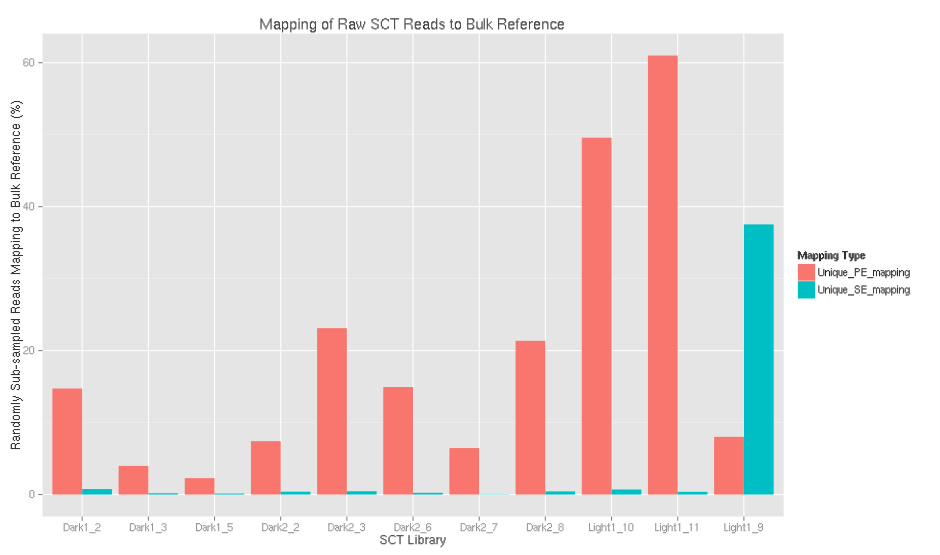
\includegraphics[width=\textwidth]{null_mapping.pdf}
    %plot of parameters random sampling and how they map 
    %null_mapping.svg
    %cutadapt vs trimmomatic plot
    \caption{Null mapping of 5000 randomly sampled PE reads from each SCT library 
                against a reference bulk transcriptome using bowtie2.
                %Of particular interest is the abnormal mapping of Light1\_9 library,
       %     where almost all reads map incongruently with their pair, despite bioanalyser
       %     traces showing fragment size selection with a clear peak at 360-385bp similarly
       % to the other libraries}
            }
    \label{fig:null_mapping}
\end{figure}




\begin{figure}[h]
    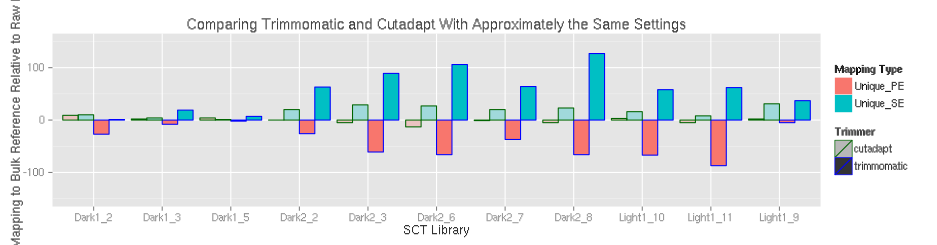
\includegraphics[width=\textwidth]{trimmomatic_vs_cutadapt.pdf}
    %plot of parameters random sampling and how they map 
    %null_mapping.svg
    %cutadapt vs trimmomatic plot
    \caption{Comparison of Trimmomatic and Cutadapt using approximately identical settings:
        specifically minimum length of 60, the entire contents of the Exeter Sequencing Service
        adapter file with respective error rate of 0.03 and Q15 for a simple match and an overall
        error threshold of Q30.

        Interestingly, cutadapt relatively increases the number of PE congruently mapping ends
        relative to untrimmed reads, whereas Trimmomatic generally leads to more PE reads mapping incongruently
        
        However, overall Trimmomatic with these settings has very slightly more paired reads mapping 
        181 vs 180.  

        The other advantages of Trimmomatic outweigh this slight performance deficit
    \label{fig:cvt}
\end{figure}



\begin{figure}[h]
    \includegraphis[width=\textwidth]{light9_insert_mapping.pdf}
\end{figure}


Scripts used to conduct this are available in my thesis scripts github repository:
\url{https://github.com/fmaguire/thesis_scripts/tree/master/chapter_2_assembly_and_binning/trimming_optimisation}




\subsection{Error correction}

Error correction of Illumina reads has been considered by some authors as a key
step in the assembly of error-correction.  This is particularly true for single-cell
data generated via MDA.


Error-correction is typically achieved by discarding lowly expressed k-mers 
as these are likely to have been generated by errors.



However, Bayeshammer as implemented in the Spades genome assembler, even on lightly trimmed
(\(Q>5\)) discarded a maximum \(0.0007\%\) of reads per 7 selected SCT libraries 
making next to no difference to final assembly.


While not optimised for SC datasets, the recommended error correction
algorithm ``seecer'' 
As there are well over 50M reads and there is no hardware restriction of memory
``seecer'' is likely the ideal error correction algorithm \citep{Macmanes2015}

DID WHAT 



\subsection{GC Partitioning of Reads}


Paired Arrangement of Reads via K-means On Unlabelled Reads (parKour).

As we expect the metagenome to contain predominantly a highly AT-rich organism, \textit{Paramecium},
(ranging from 24.1 to 28.2\%GC in \textit{P. aurelia} species complex and \textit{P. caudatum} \citep{Aury2006,McGrath2014})
and a very GC-rich organism, \textit{Micractinium}, (\textit{Chlorella variabilis} NC64A genome is approximately 67.1\%GC, the highest
found in a sequenced eukaryote genome (in 2010) \citep{Blanc2010}).

Although intriguingly low-GC regions 55-65\%GC have a significantly higher number of mapped genes suggesting they are highly expressed \citep{Blanc2010}

Also correlations with increased GC richness in highly expressed regions of paramecium

Therefore,  would be closer than whole genome richness but still separable, this can be seen in the bimodal GC distribution in the raw and trimmed sequencing 
reads.

\begin{figure}
    Example GC plot showing bimodal distribution
\end{figure}

Due to the difficulties generating a high quality \textit{de novo} metatranscriptome assembly, I considered  it worth investigating whether there could be GC\%
clusters and furthermore whether assigning reads to these clusters and assembling the reads corresponding to a cluster would generate any meaningful groupings of reads.

To this end, I 

parKour:
\begin{enumerate}
    \item Parse user input of paired FASTQ files corresponding to Forward and Reverse Paired-End reads, and desired number of clusters
    \item Simultaneously iterate over the pair of FASTQ files calculating the GC\% for each loading results into an Armadillo \(2xN\) matrix where \(N\) is the total number of PE reads
    \item MLPACK K-means clustering:
        \begin{itemize}
            \item \
        \end{itemize}
    \item 
    \item Re-read the two input FASTQs assigning them to output files based on the assigned cluster of the pair
\end{enumerate}



Scripts used to conduct this are available in a github repository:
\url{https://github.com/fmaguire/parKour}



\subsection{Assembly}

Trinity uber alles



\begin{table}[h]
\begin{tabular}{|l|rrrrrrrl}
\hline
\multicolumn{1}{|c|}{Assembly} & \multicolumn{1}{c|}{Raw Reads (paired)} & \multicolumn{1}{c|}{\begin{tabular}[c]{@{}c@{}}Trimmed Reads \\ (assuming all paired)\end{tabular}} & \multicolumn{1}{c|}{Assembled Contigs} & \multicolumn{1}{c|}{Assembled "Genes"} & \multicolumn{1}{c|}{"Gene" N50} & \multicolumn{1}{c|}{"Gene" Mean Length} & \multicolumn{1}{c|}{"Gene" Total Assembled Bases} & \multicolumn{1}{c|}{GC\%} \\ \hline
Kodama Trinity                 & 232.3M                                  & 218.5M                                                                                              & 68,175                                 & 40,805                                 & 904                             & 1,832                                   & 36.9M                                             & \multicolumn{1}{c}{?}     \\ \cline{1-1}
SCT Q30                        & 126.9M                                  & 93.2M                                                                                               & 99,784                                 & 88,573                                 & 475                             & 451                                     & 40.0M                                             & 48.67                     \\ \cline{1-1}
SCT Q30 + Bulk                 & 179.4M                                  & 145.6M                                                                                              & 127,508                                & 103,506                                & 646                             & 564                                     & 58.2M                                             & 40.30                     \\ \cline{1-1}
SCT Q5                         & 126.9M                                  & 108.2M                                                                                              & 112,182                                & 99,441                                 & 465                             & 447                                     & 44.5M                                             & 49.42                     \\ \cline{1-1}
SCT Q5 + Bulk                  & 179.4M                                  & 160.6M                                                                                              & 139,226                                & 113,685                                & 615                             & 549                                     & 62.5M                                             & 41.28                     \\ \cline{1-1}
Bulk                           & 52.4M                                   & 52.4M                                                                                               & 43,261                                 & 30,706                                 & 1264                            & 861                                     & 26.5M                                             & 29.61                     \\ \cline{1-1}
\end{tabular}
\end{table}



\subsubsection{Comparing assemblers}
Trinity,
SOAP de novo Trans
TransAbyss
Velvet+Oases

Trinity best

\subsubsection{Optimising Trinity Assembly}

minkmer cov 2: yay or nay

Error correction: yay or nay

Digital normalisation: yay or nay

\subsubsection{Assembly assessment}
CEGMA - not perfect for genomic - numbers are not directly as the transcriptome metabolic and cellular function
genes will be overrpretented 
RSEM-eval
Mapping percentage


Assembly parameters e.g. N50, transcript number, total bp assembled are not necessarily useful
as wildly different valuesreturn similar gene content \citep{Lowe2014}
These parameters have been demonstrated as being inconsistent for test ``perfect assemblies'' 





After assembly transcripts shorter than 200bp were removed and CD-HIT was sued to elimiate small 
transcripts with 99\% idendity to longer transcripts  ``cd-hit-est -i TREANSCRIT -c 0.99 -o Ol:UTPU''


Trinity assemblies have been found to include more low-abundance k-mers than oases, many different isoforms
but doesn't recover many more unique genes just more isoforms \citep{Lowe2014} 

k-mer spectrum can be used to evaluate reocvoeery of low-abundance transcrtipts \citep{Pop2009}



\section{ORFs calling}

Too many transcripts 

Universal or tetrahymena genetic code.

The ciliate code reassigns 2 universal stop codons (UAA, UAG) to Gln amab





ORFs were extracted from transcriptome using transdecoder and a minimum protein size of 50aa
because


\section{Binning}
For this purpose ete2 library was ported to python3 (pull request outstanding to merge this into ete2 codebase)


\subsection{Dendrogenous}
Phylogeny generation

\subsection{Arboretum}
Binner 

Training data manually parsed



\section{Saturation}
Estimating saturation can only be done after binning as we are only interested in host and algal endosymbiont
So saturation on binned contigs.





